% Created 2023-06-18 Κυρ 18:59
% Intended LaTeX compiler: pdflatex
\documentclass[11pt]{article}
\usepackage[utf8]{inputenc}
\usepackage[T1]{fontenc}
\usepackage{graphicx}
\usepackage{longtable}
\usepackage{wrapfig}
\usepackage{rotating}
\usepackage[normalem]{ulem}
\usepackage{amsmath}
\usepackage{amssymb}
\usepackage{capt-of}
\usepackage{hyperref}
\usepackage{minted}
\usepackage[utf8]{inputenc}
\usepackage[LGR]{fontenc}
\usepackage[T1]{fontenc}
\usepackage[english, greek, american]{babel}
\author{Torosian Nikolas}
\date{\today}
\title{Thermodynamics\\\medskip
\large notes}
\hypersetup{
 pdfauthor={Torosian Nikolas},
 pdftitle={Thermodynamics},
 pdfkeywords={},
 pdfsubject={},
 pdfcreator={Emacs 28.2 (Org mode 9.6.1)}, 
 pdflang={English}}
\begin{document}

\maketitle
\tableofcontents

\section{Energy}
\label{sec:orgef812e4}
\subsection{Special esoteric energy}
\label{sec:org135c66b}
\begin{equation}
\begin{align}
\bar u = \frac{U}{m} \ [\right\frac{J}{kg}\left], \\
&m = mass \\
&U = energy \\
\end{align}
\end{equation}

\section{density}
\label{sec:org4d6a31b}

\begin{equation}
\begin{align}
p= \frac{m}{V}
\end{align}
\end{equation}

\section{Special Volume}
\label{sec:orgc02aa26}
Opposite of density
\begin{equation}
\begin{align}
\bar v = \frac{m}{V}
\end{align}
\end{equation}
\section{properties of clean solutions in thermodynamix by Katsap}
\label{sec:org4da8ef8}

\subsection{hydrated/dehydrated steam\hfill{}\textsc{example1}}
\label{sec:org75b23d9}

\selectlanguage{greek}
\subsubsection{Υδρατμοι 20 \%}
\label{sec:orgb981b4c}
\subsubsection{Πιεση}
\label{sec:orgbc43471}
\selectlanguage{english}
150 kPa
\begin{enumerate}
\item solution\hfill{}\textsc{example1}
\label{sec:org36facdb}
\selectlanguage{greek}

Απο πίνακες πρεπει να τα βρίσκω όλα \ldots{}

για να μπορέσω να τα βρώ θέλω τον σωστό πίνακα\ldots{}..

\begin{center}
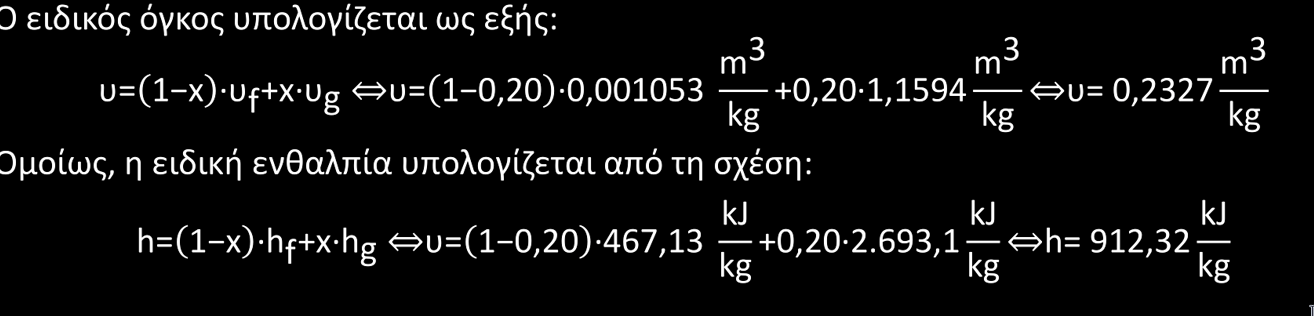
\includegraphics[width=.9\linewidth]{/home/dtos_experiment/Documents/univercity/thermodynamics/hydrted-steam-solution.png}
\end{center}
\selectlanguage{english}
\end{enumerate}
\subsection{coolant enthalpy\hfill{}\textsc{example2}}
\label{sec:orgfd071ef}
\subsubsection{20 kg (R134a)}
\label{sec:org82575cc}
\subsubsection{air composition 85\%}
\label{sec:orgb5079e9}
\subsubsection{heated at 90 °C}
\label{sec:org0c70943}
\subsubsection{constant pressure 1MPa}
\label{sec:org098aaa8}
\begin{enumerate}
\item solution\hfill{}\textsc{example2}
\label{sec:orgc8b353b}
\begin{enumerate}
\item go to tables
\item find all needed stuff
\(u_{f},...,h_{f}\)
\item solve the God damn thing by:
\begin{enumerate}
\item plugin the values
\item u and h have the same general equation. (see example1)
\end{enumerate}
\item x is always the (\%) given in the known states of the system.
\item go in the P/H diagram and cross-find special enthalpy
\(h_{2}\)
\item solve the easyest  equation
\(\Delta(H) = \Delta(h) \cdot m\)
\end{enumerate}
\end{enumerate}
\subsection{overheated steam\hfill{}\textsc{example3}}
\label{sec:orgdf0e6ef}
\subsubsection{Pressure \(P_{g}\) = 1,5 \([(MNt)/m^2]=[MPa]\)}
\label{sec:org05df083}
\subsubsection{degrees Of Heating \(\Theta\)  = 76,7 °C}
\label{sec:orgfee55bf}
\begin{enumerate}
\item solution\hfill{}\textsc{example3}
\label{sec:orga4cd880}
\begin{enumerate}
\item degrees Of Heating == \(\Theta\) °C \(\uparrow\)+ \(T_{sat}\)( °C ) at 1,5 \(MPa\)
\item Linear interpolation  for T1 and T2 at \(P_{g}\), where \(P_{g}\) \(\in\)\{P1<P<P2\}

\selectlanguage{greek}
(γραμμική παρεμβολή)
\selectlanguage{english}

\item find the mean value T
\((T_{n}-T_{n-1})/n\)
\item for \(h\)
\begin{enumerate}
\item calculate \(h\) for P1 and P2 in the respective for T

Where T1<
T=°C \(\uparrow\)+ Tκορ(°C) σε 1,5 \(MPa\)
<T2

\item compute the lin. interpolation for \(h\) at T (see (1.))
\begin{center}
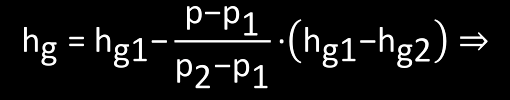
\includegraphics[width=.9\linewidth]{/home/dtos_experiment/Documents/univercity/thermodynamics/triple-lin-interpol.png}
\end{center}
\end{enumerate}
\end{enumerate}
\end{enumerate}
\section{1st law of thermodynamix by Katsap}
\label{sec:org4677984}
\subsection{dencity and special volume}
\label{sec:org03c247e}
\begin{equation}
\begin{align}
d = \frac{1}{u} \\
where\ u &= \frac{V}{m} \\
&= \frac{\dot{V}}{\dot{m}} \\
\end{align}
\end{equation}
\subsection{mass/volume supply}
\label{sec:org06c7368}

\begin{center}
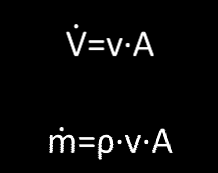
\includegraphics[width=250px,height=140px]{/home/dtos_experiment/Documents/univercity/thermodynamics/supply-equations.png}
\end{center}
\end{document}